%
% ELEMENTOS DUNHA OBRA DE ARTE MUSICAL: MATERIA PRIMA - SON
% ---------------------------------------------------------
%\subsection{O son como materia prima} \label{sub:elementos-obra-arte}

Co�ecida a complicaci�n de definir a m�sica, e antes de adentrarnos en profundidade nas s�as orixes, conv�n co�ecer os elementos que integran unha <<obra de arte>> musical e aqueles que teremos en conta para achegarnos a ela.

\begin{Figura}
    \centering
    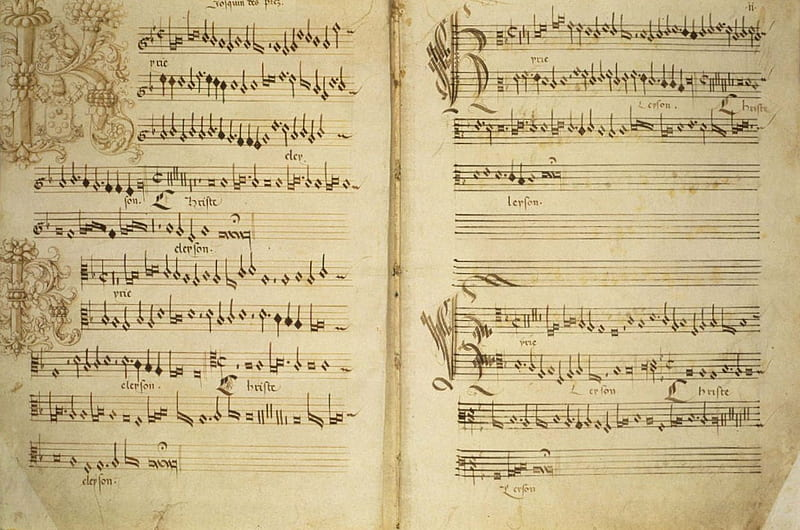
\includegraphics[width=0.9\textwidth]{../figures/ud-00/partita-vella.jpg}
    \captionof{figure}{Representaci�n gr�fica da obra de arte musical}
    \label{fig:partita-vella}
\end{Figura}

O elemento principal ou a materia prima da que partimos para analizar unha obra de arte musical � o \textbf{son},
\sidenote{sensaci�n producida no o�do polas vibraci�ns dos corpos el�sticos, propagados a trav�s do aire.}
que ven definido pola altura, intensidade, timbre e duraci�n. Ac�sticamente definiremos estes conceptos do seguinte xeito:

\begin{caja}[PROPIEDADES DO SON]
    \begin{description}\label{propiedades-son}
    \item
    [Altura]: ven determinada polo n�mero de vibraci�ns por segundo, isto � a frecuencia. Maior frecuencia $\Rightarrow$ sons m�is agudos, e menor frecuencia $\Rightarrow$ sons m�is graves.
    \item
    [Intensidade]: ven determinada pola amplitude de onda da vibraci�n. Maior amplitude $\Rightarrow$ sons fortes e menor amplitude $\Rightarrow$ sons m�is suaves.
    \item
    [Timbre]: depende da cantidade de harm�nicos que te�a un son e da intensidade de cada un deles; esta caracter�stica � a que diferencia principalmente voces e instrumentos.
    \item
    [Duraci�n]: ven definida como a persistencia da onda sonora no tempo. Maior duraci�n $\Rightarrow$ sons m�is longos e vicecersa.
    \end{description}
\end{caja}

A representaci�n gr�fica de todas estas propiedades est� expresada nos diferentes sistemas de notaci�n e foi dende sempre, algo perseguido polos te�ricos da m�sica ao longo da historia.





